% vim: tw=80

\chapter{Introduction}

Modern particle physics is driven by the desire to answer the questions about the
fundamental constituents of matter and the principles of interaction between
them. High-energy collisions of particles and the analysis of their
scattering products are an optimal method to gain deep insights into the
fundamental principles of the universe. 

In hadron-hadron collisions at the LHC, point-like parton-parton scattering can
produce outgoing partons with large transverse momenta. The outgoing partons
manifest themselves as a spray of collimated particles, which are clustered
together into so-called \emph{jets}. Events containing two such jets with large
transverse momenta, dijet events, allow for rigorous tests of perturbative
Quantum Chromodynamics (pQCD) predictions and can subsequently also be used to
gain a better understanding of the inner structure of the proton and to
determine the strong coupling constant.

Especially in view of upcoming NNLO corrections for dijet calculations in
perturbative QCD, dijet observables are an optimal candidate for precision
studies of the proton. Consequently, such event topologies were studied and an
ideal observable was found in the triple-differential dijet cross section.

This thesis presents the theoretical motivation and the data analysis of the
triple-differential dijet cross section, which is measured as a function of the
average transverse momentum of the two leading jets and is binned in the
rapidity separation and the boost of the dijet system.
Figure~\ref{fig:intro_ybys_hint} illustrates the various dijet combinations as
they are accesible in this measurement. Since different momentum fractions of
the proton are accessed in these bins, this measurement optimally relates the
dijet cross section to the underlying momentum fractions of the proton. This is
demonstrated thereupon by a combined fit of the proton PDFs to deep-inelastic
scattering data from the HERA experiments and the triple-differential dijet
cross section.

\begin{figure}[h!tb]
    \centering
    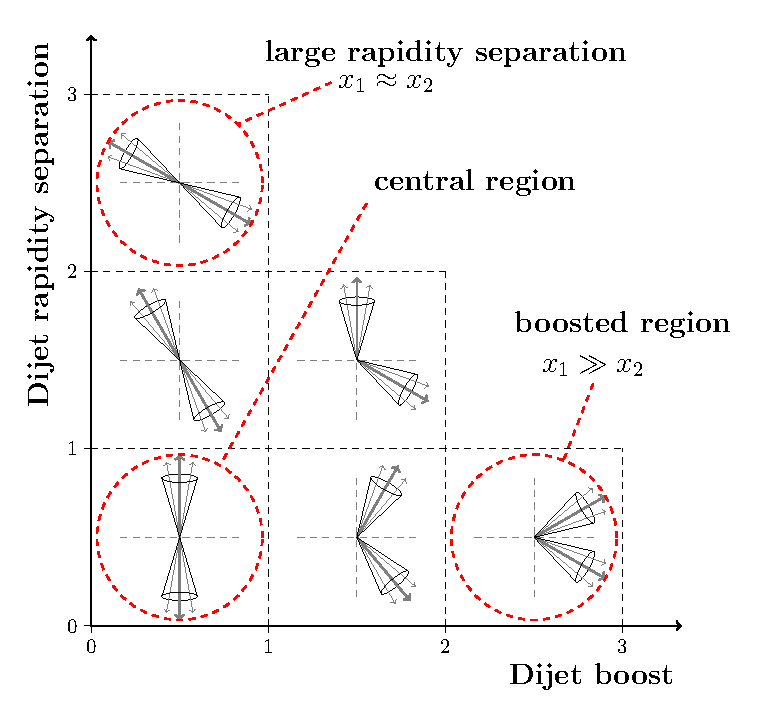
\includegraphics[width=0.6\textwidth]{figures/drawings/ybys_hint.pdf}
    \caption{A depiction of dijet topologies in the \ystar and \yboost bins.
             Same-side and opposite-side dijet events are separated into
             different bins, which allows to draw conclusions about the proton
             PDFs as different fractional proton momenta are accessed.}
    \label{fig:intro_ybys_hint}
\end{figure}

In Chapter~\ref{sec:theoretical_foundations}, the theoretical foundations for
jet production at hadron-hadron colliders are outlined. An overview of the
Standard Model of particle physics with a focus on perturbative quantum
chromodynamics is given. Additionally, the relativistic kinematic of dijet
production is explained. Chapter~\ref{sec:experimental_setup} summarizes the
experimental setup of the LHC collider and the CMS detector. The
employed software tools and Monte Carlo event generators are described.

The theoretical motivation and the definition of the observables are introduced
in Chapter~\ref{sec:theory_predictions}, in which also the accuracy of the NLO
pQCD calculation is studied. The measurement of the triple-differential dijet
cross section with data of the CMS experiment is explained in
Chapter~\ref{sec:measurement} starting with the event and jet selection to
guarantee clean dijet events. The measurement is scrutinized using a multitude
of studies regarding the detector and reconstruction efficiency. It is corrected
for detector effects in an unfolding procedure and is compared to NLO
predictions calculated in pQCD.

Finally, the sensititivity of the proton PDFs to the measured data is
demonstrated in Chapter~\ref{sec:pdf_constraints} resulting in constraints on
the PDFs, especially the gluon PDF. Moreover, a simultaneous fit of the PDFs and
the strong coupling constant is presented.

% \layout
